% Begin your document as any latex file
\documentclass{article}[a4paper]
% Use package 6895
\usepackage{6895}
\usepackage[utf8]{inputenc} % 'cp1252'-Western, 'cp1251'-Cyrillic, etc.
\usepackage[english]{babel} % 'french', 'german', 'spanish', 'danish', etc.
\usepackage{amsmath}
\usepackage{amssymb}
\usepackage{txfonts}
\usepackage{mathdots}
\usepackage[classicReIm]{kpfonts}
\usepackage{graphicx}

% The following are just for the sake of this document.  Ignore them
% for the purposes of generating scribe notes.
% --------------------------------------------------------------------
\newcommand{\pc}[1]{{\tt\begin{description} \item [\TT] #1
\end{description}}}

\newcommand{\com}[1]{$\backslash$#1}
\newcommand{\comone}[2]{$\backslash$#1\{#2\}}
\newcommand{\comtwo}[3]{$\backslash$#1\{#2\}\{#3\}}
\newcommand{\comthree}[4]{$\backslash$#1\{#2\}\{#3\}\{#4\}}
\newcommand{\comfour}[5]{$\backslash$#1\{#2\}\{#3\}\{#4\}\{#5\}}
\newcommand{\comfive}[6]{$\backslash$#1\{#2\}\{#3\}\{#4\}\{#5\}\{#6\}}

\newcommand{\sh}[2]{\com{#1} & $#2$ \\}
\newcommand{\shn}[2]{\com{#1} & #2 \\}

\newenvironment{todolist}{\begin{description}}{\end{description}}
\newcommand{\todoitem}[2]{\item {\em #1} \hfill \\ #2}
% ---------------------------------------------------------------------

% Begin the lecture with a line like the following:
% This replaces the usual \begin{document} that a latex
% file begins with.
%\begin{lecture}{0}{How to Do Scribe Notes}{Seth Gilbert}
\begin{lecture}{Winter semester 2023/24}{Multiple access techniques used for satellite communications}{Agarwal (1428490)}
% Now summarize the lecture.  This should be like an abstract
% for the lecture, broken down into a few bullet points.
\textbf{\textit{Abstract}: This project report provides a comprehensive overview of the fundamentals, characteristics, architecture, advantages, and disadvantages of Multiple Access (MA) techniques employed in satellite communications. The challenge of facilitating simultaneous communication among numerous single or multipoint mobile satellite users is addressed through MA methods, including \textit{Frequency Division Multiple Access (FDMA), Time Division Multiple Access (TDMA), Code Division Multiple Access (CDMA), Space Division Multiple Access (SDMA), and Random (Packet) Division Multiple Access (RDMA)}. Due to limitations in system resources such as transmitting power and bandwidth, optimal utilization involves assigning complete channels to different MAs. This, however, introduces complexities in signal summation and separation during transmission and reception processes, respectively.}

% Now organize your lecture into sections.
\section{Introduction}
\seclabel{Intro}

Due to the vast progress in the field of satellite communications, information transmission, as well as communication across vast distances, is possible seamlessly with larger user-handling capacity and minimal operational costs. Satellite Communications allow multiple users to share and exchange information simultaneously with optimal bandwidth allocation. Therefore, it is possible that multiple carriers from multiple earth stations are accessing the mobile or fixed Satellite without interference, and the transponder of the satellite is loaded with multiple carriers. This type of access technique in satellite communication is known as \textit{Multiple access technique}. The multiple carriers can be from different geographically apart earth stations and each earth station can transmit one or more signals. Multiple Access techniques play a vital role in increasing the efficiency and utilizing the resources of the satellite and providing several services such as broadcasting, telecommunications, etc.


However, if the satellite transponder’s channel is only loaded with a single transmission carrier, then this technique is known as \textit{Single Access Technique}. Nowadays, the single-access technique is not frequently used due to its high operational costs.


This project report gives insight into various multiple access (MA) techniques used in Satellite communication, their advantages, and disadvantages as well. The following five MA techniques are used in Satellite communication:
\begin{enumerate}
\item  \textbf{Frequency Division Multiple Access (FDMA):} FDMA assigns each relevant Earth Station, a distinct working carrier Radio Frequency (RF) within the spacecraft transponder bandwidth as shown in \figref{fig:MA}(a).

\item  \textbf{Time Division Multiple Access (TDMA):} All stations share the same frequency and bandwidth, but they take turns transmitting in non-overlapping time slots as shown in \figref{fig:MA}(b).

\item  \textbf{Code Division Multiple Access (CDMA):} CDMA allows all relevant Earth stations to simultaneously share the same bandwidth, distinguishing signals through various processes, such as code identification as shown in \figref{fig:MA}(c). It involves sharing both frequency and time resources using mutually orthogonal codes, like a Pseudorandom Noise (PN) sequence.

\item  \textbf{Space Division Multiple Access (SDMA):} SDMA enables all relevant Earth stations to use the same RF simultaneously within a distinct space allocated for each link. In SDMA, the frequency reuse concept is used in which the transponders are connected to separate spot-beam antennas while working to operate at the same frequency.

\item  \textbf{Random (Packet) Division Multiple Access (RDMA): }RDMA is a scheme where many satellite users asynchronously share the same transponder by randomly transmitting short bursts or packet divisions.\cite{Ilcev2013}
\end{enumerate}

\begin{figure}[!h]
\center
  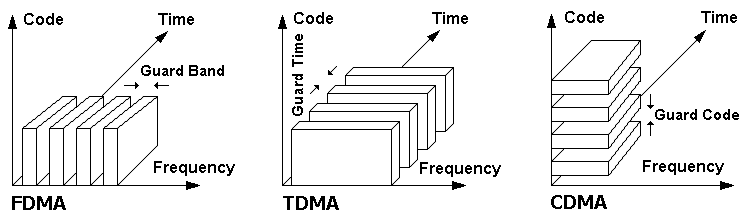
\includegraphics[scale=0.4]{image1}
  \caption{The concepts of multiple access: (a) FDMA; (b) TDMA; (c) CDMA.\cite{Ilcev2005}}
  \figlabel{fig:MA}
\end{figure}
%\includegraphics*[width=6.19in, height=1.78in]{image1}

Different methods exist for classifying multiple access (MA), and one such classification is based on how circuits are allocated to users. Here, ``circuits" refers to individual communication channels through the multiple-access transponder. Circuits can be categorized as \textbf{\textit{preassigned}}, indicating that they are designated on a fixed or partially fixed basis for specific users, irrespective of traffic fluctuations. These circuits are not open for general use and are reserved for the allocated users. While pre-assignment is a straightforward approach to implement, its efficiency is most pronounced when dealing with circuits experiencing continuous and substantial traffic. Therefore, this approach is well-suited for communication links experiencing substantial traffic exchange between receivers (Rx) and transmitters (Tx).

Instead of pre-assignment, an alternative approach is \textbf{\textit{Demand-Assigned Multiple Access (DAMA)}}\textit{.} In DAMA, all circuits are accessible to every user and are allocated based on demand. While DAMA leads to a more efficient overall utilization of circuits, it tends to be more expensive and complex to implement. Both FDMA and TDMA systems can function as either preassigned or demand-assigned systems. In contrast, CDMA operates as a \textbf{\textit{random-access system}}, lacking control over the timing of access or the frequency slots accessed.\cite{Ilcev2013,Roddy423}

\section{Frequency Division Multiple Access (FDMA)}
\seclabel{FDMA}

The FDMA concept is the most prevalent and initial multiple access scheme used in satellite communication systems. The repeater channel's bandwidth is segmented into sub-bands, each allocated to a carrier transmitted by earth stations. In this access method, earth stations transmit continuously, and the channel concurrently carries multiple carriers at distinct frequencies. To prevent interference due to imperfections in oscillators and filters, guard intervals between each carrier-occupied band are essential.


The receiver selects the desired carrier based on the appropriate frequency, facilitated by the intermediate frequency (IF) amplifier for filtering. The downlink receiver (Rx) chooses the necessary carrier based on the appropriate radio frequency (RF). When the satellite transmitter (Tx) is operating near saturation, nonlinear amplification generates intermodulation (IM) products that might interfere with other users' signals. To minimize IM, it's crucial to run the transponder with reduced total input power, following input back off, and ensure sufficient filtering by the intermediate frequency (IF) amplifier.


Therefore, FDMA assigns a single satellite channel to one mobile user at a time. In case of a degraded transmission path, the controller switches the system to another channel. While technically straightforward, FDMA is inefficient in terms of bandwidth usage because it assigns a voice channel to a single conversation, irrespective of whether someone is speaking. Additionally, it can't accommodate diverse forms of data, only voice transmissions. Despite these limitations, FDMA persists due to its proven reliability and simplicity, remaining a widely used approach.\cite{Ilcev2013,Maral284}

\subsection{Hybrid Transmission Schemes}
\seclabel{Hyb-Sch}

Depending on the employed multiplexing and modulation techniques, various transmission hybrid schemes can be explored. Generally, these can be categorized into two groups, considering the traffic demands on Multiple Channels per Carrier (MCPC) and Single Channel per Carrier (SCPC) by Earth stations.

\begin{enumerate}
\item\textbf{Multiple Channels per Carrier (MCPC):} It involves essential components such as a multiplexer, modulator, and transmitter through a satellite uplink. The multiplexed data undergo modulation and are then transmitted to an allocated Radio Frequency (RF) segment. This approach is particularly employed when the transponder's bandwidth is shared among several Earth Station units, each with distinct traffic requirements.

The transponder's bandwidth is partitioned into fixed segments, each assigned to SES units with specific time-frequency divisions. Guard bands are inserted between these segments to mitigate interference, but this leads to reduced bandwidth utilization efficiency. The extent of this loss is directly proportional to the number of accessing SES units in the network. The total number of carriers passing through the satellite transponder depends on the number of receiving SES units.\cite{Ilcev2013}

\item\textbf{Single Channel per Carrier (SCPC): }In certain scenarios, like providing digital services to remote areas or individual Earth Station with low traffic demands, assigning multiple channels to each Earth Station is inefficient as most channels remain unused for a significant part of the day. For such applications, the SCPC type of FDMA is employed. In the SCPC system, each carrier is modulated by only one voice or a low to medium-bit rate data channel.\cite{Ilcev2013}
\end{enumerate}

\noindent There are several combinations of multiplexed FDMA integrated with SCPC, PSK, and TDM techniques:

\begin{enumerate}
\item  \textbf{SCPC/FDMA: }The baseband signals at the earth station modulate individual carriers separately. This is referred to as a single connection per carrier (SCPC). Each carrier accesses the satellite repeater channel on its specific frequency simultaneously with other carriers from the same or different stations. Information routing is thereby conducted based on the 'one carrier per link' principle.\cite{Maral284}

\item  \textbf{TDM/PSK/FDMA: }The digital baseband signals originating from the earth station are amalgamated to create a Time Division Multiplexing (TDM) signal. This multiplexed signal, represented by a binary stream, modulates a carrier through Phase Shift Keying (PSK), gaining access to the satellite repeater channel at a specific frequency. This occurs simultaneously with other carriers from various stations on different frequencies. To minimize intermodulation products, and thereby reduce the number of carriers, traffic routing ideally follows the 'one carrier per transmitting station' principle. The TDM signal encompasses all traffic from the transmitting earth station to every other station.\cite{Maral284}
\end{enumerate}

\subsection{Adjacent Channel Interference}
\seclabel{ACI}

As depicted in \figref{ACI}, the channel bandwidth accommodates multiple carriers across different frequencies. These carriers are transmitted to all the earth stations within the satellite antenna's coverage area. Each earth station's receiver must filter these carriers, and effective filtering is achievable when the carrier spectra are distinctly separated by a broad frequency guard band. However, opting for wider guard bands results in inefficient utilization of the channel bandwidth and increased operational costs per carrier for the space segment. Therefore, a technical and economic compromise is necessary. Regardless of the chosen compromise, a portion of the power from a carrier adjacent to a specific carrier will be received by the receiver tuned to the frequency of the considered carrier. This phenomenon introduces noise in the form of interference, known as adjacent channel interference (ACI).\cite{Maral285}

\begin{figure}[!h]
\center
  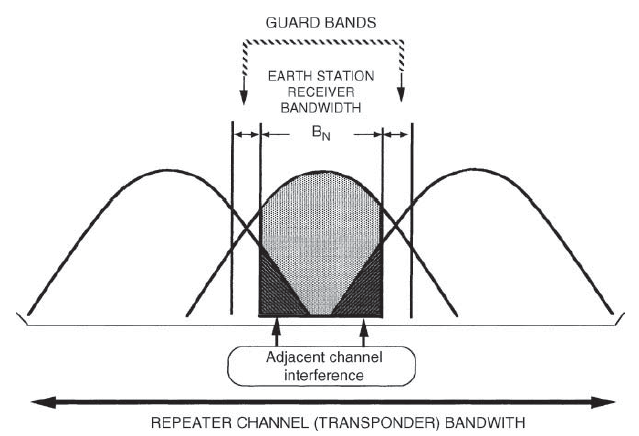
\includegraphics[scale=0.7]{image2}
  \caption{Adjacent channel interference in FDMA.\cite{Maral285}}
  \figlabel{ACI}
\end{figure}

\subsection{Intermodulation}
\seclabel{IM}

\noindent The satellite repeater channel exhibits a nonlinear transfer characteristic. In the context of FDMA, this channel amplifies multiple carriers simultaneously, each at different frequencies. The earth station is equipped with a nonlinear power amplifier, which can receive signals from multiple carriers at varying frequencies. Generally, when N sinusoidal signals with frequencies f${}_{1}$, f${}_{2}$, {\dots}, f${}_{N}$ go through a nonlinear amplifier, the output contains not only the N signals at their original frequencies, but also undesired signals known as intermodulation products. These products manifest at frequencies f${}_{IM}$, which are linear combinations of the input frequencies, expressed as:
\begin{equation}
f_{IM}=m_1f_1+m_2f_2+.......+m_Nf_N
\end{equation}
where, m${}_{1}$, m${}_{2}$, {\dots}, m${}_{N}$ are positive or negative integers.

\noindent The term X represents the order of an intermodulation product, determined by the expression:
\begin{equation}
X=|m_1|+|m_2|+......+|m_N|
\end{equation}
In scenarios where the centre frequency of the passband amplifier is considerably larger than its bandwidth, as is typical for a satellite repeater channel (with a centre frequency in the several GHz range and a bandwidth in the few tens of MHz range), only odd-order intermodulation products, where $\Sigma$m${}_{i}$ = 1, are contained within the amplifier bandwidth. Additionally, the amplitude of intermodulation products diminishes with the order of the product. Consequently, in practical applications, only products of order 3, and to a lesser extent 5, hold significance. \figref{IM} illustrates the generation of intermodulation products from two unmodulated carriers at frequencies f${}_{1}$ and f${}_{2}$. Notably, in the case of unmodulated carriers of unequal amplitude, intermodulation products are more pronounced at higher frequencies if the carrier of greater amplitude has a higher frequency and at lower frequencies if the carrier of greater amplitude has a lower frequency. This underscores the advantage of siting the most powerful carriers at the extremes of the channel bandwidth, ensuring that the corresponding potent intermodulation products fall outside the channel bandwidth and do not propagate on the downlink.\cite{Maral286}

\begin{figure}[!h]
\center
  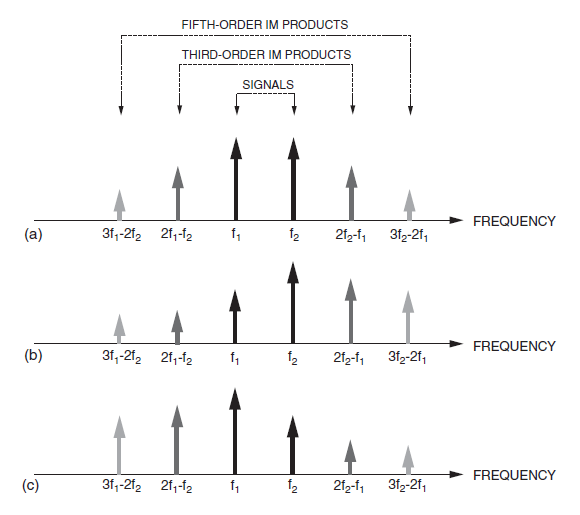
\includegraphics[scale=1]{image3}
  \caption{Intermodulation products in the scenario of two sinusoidal signals (unmodulated carriers): (a) with equal amplitudes; (b) and (c) with unequal amplitudes.\cite{Maral286}}
  \figlabel{IM}
\end{figure}

\subsection{Shortcomings of FDMA}
\seclabel{Short_FDMA}

\noindent FDMA is identified by continuous access to the satellite within a specific frequency band. While this approach offers simplicity and does not require synchronization between earth stations, it comes with certain drawbacks:

\begin{enumerate}
\item  Limited flexibility during reconfiguration. Adapting to changes in capacity requires altering the frequency plan, necessitating modifications to transmitting and receiving frequencies, as well as filtering bandwidths of the earth stations.

\item  Capacity loss as the number of accesses increases due to the generation of intermodulation products, demanding operation at reduced satellite transmitting power (back-off).

\item  The necessity to regulate the transmitting power of earth stations to ensure equal carrier powers at the satellite input, preventing the capture effect. This control must be real-time and adaptable to attenuation caused by rain on the uplinks. In telecommunications, the capture effect, or frequency modulation (FM) capture, is a phenomenon associated with FM reception where only the stronger of two signals at, or near, the same frequency or channel will be demodulated.\cite{Maral289}
\end{enumerate}

\section{Time Division Multiple Access (TDMA)}
\seclabel{TDMA}
In this MA technique, only one carrier utilizes the transponder at any given moment, eliminating intermodulation products resulting from the nonlinear amplification of multiple carriers. As only one TDMA burst occupies the entire RF bandwidth of the satellite transponder at any given time, there is no need for input back off in TDMA, unlike in FDMA where it is required to reduce interference from intermodulation. This presents a notable advantage of TDMA, allowing the transponder’s traveling wave tube (TWT) to operate at maximum power output or saturation level. As TDMA involves transmitting signal information in bursts, it is well-suited for digital signals. Digital data can be organized into burst format for transmission and reassembled from the received bursts using digital buffer memories.

\figref{Burst} illustrates the fundamental TDMA concept, where stations transmit bursts sequentially. Synchronization of bursts is necessary, and in the depicted system, one station is exclusively assigned to transmit reference bursts to which others synchronize. The time interval from the start of one reference burst to the next is termed a \textit{frame}, encompassing the reference burst R and bursts from other earth stations, denoted as A, B, and C in \figref{Burst}. Another reference burst might succeed the initial one to offer redundancy. Various synchronization techniques, including random access, open-loop, and closed-loop, have been suggested to enhance the imperfect timing of TDMA bursts in a systematic manner.\cite{Ilcev2013,Roddy436}

\begin{figure}[!h]
\center
  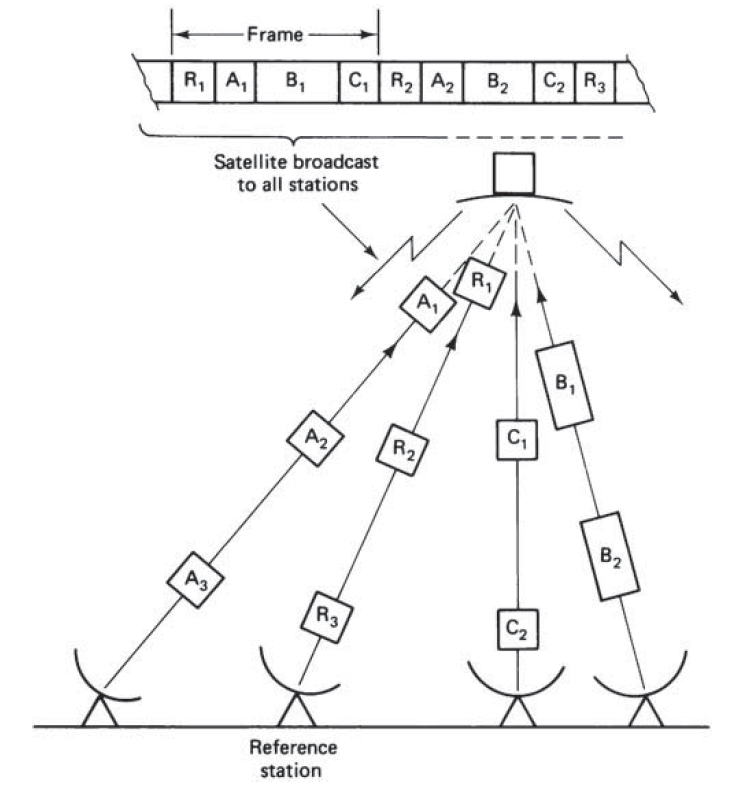
\includegraphics[scale=0.6]{image4}
  \caption{Burst Synchronization in TDMA with a reference Station.\cite{Roddy436}}
  \figlabel{Burst}
\end{figure}

\noindent Given the frame time interval T${}_{F}$ and input bit rate R${}_{b}$ considering the burst transmission as continuous and for a single channel, the necessary buffer capacity M can be expressed as
\begin{equation}
M=R_bT_F
\end{equation}
The buffer memory is filled at the input bit rate R${}_{b}$ within the frame time. Subsequently, these M bits are transmitted as a burst in the following frame, ensuring a seamless continuity of the input. The set of M bits is transmitted during the burst time T${}_{B}$, and the transmission rate, equivalent to the burst bit rate, is denoted as
\begin{equation}
R_{TDMA}=\frac{M}{T_B}=R_b\frac{T_F}{T_B}
\end{equation}
\cite{Roddy436}
\subsection{Basic equipment units in a TDMA ground station}
\seclabel{euip_TDMA}

\noindent \figref{Unit} illustrates key components within a TDMA ground station, designated as Earth Station A for explanatory purposes. Digital traffic from terrestrial links entering Earth Station A is directed to destination stations labeled B, C, and X. Assuming consistent bit rates for the digital traffic on each terrestrial link, the \textit{terrestrial interface modules (TIMs)} convert incoming continuous-bit-rate signals into intermittent-burst-rate mode. These individual burst-mode signals undergo time-division multiplexing in the \textit{time division multiplexer (MUX)}, ensuring that the traffic for each destination station is allocated to its designated time slot within a burst. Specific time slots at the start of each burst are utilized for transmitting timing and synchronizing information, collectively referred to as the \textit{preamble}. The entire burst, encompassing the preamble and traffic data, is employed for phase modulating the radio frequency (RF) carrier.

The signal received at an earth station comprises bursts from all transmitting stations, organized in the frame format detailed in \secref{Frame_format} of this project report. The RF carrier undergoes conversion to an intermediate frequency (IF) before demodulation. A dedicated \textit{preamble detector} supplies timing details for both the transmitter and receiver, along with a carrier synchronizing signal for the phase demodulator.\cite{Roddy436}

\begin{figure}[!h]
\center
  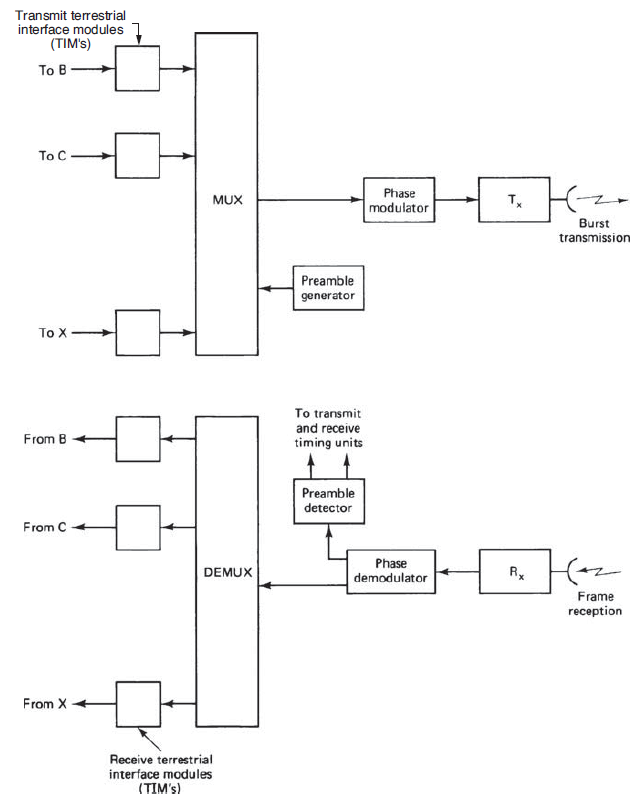
\includegraphics[scale=1]{image5}
  \caption{Basic Equipment units in a TDMA ground station.\cite{Roddy436}}
  \figlabel{Unit}
\end{figure}

\subsection{Frame and Burst Format in a TDMA System}
\seclabel{Frame_format}

\noindent A frame consists of several bursts from different transmitting stations. As shown in \figref{Burst_Format}, the first frame consists of a reference burst and the subsequent frames consist of several traffic bursts from different transmitting stations such as Station A, B, {\dots}., Y, and Z.

\textbf{Reference Burst: }The reference burst signals the start of a frame is divided into individual time slots or channels and is essential at the commencement of each frame to supply timing details for acquiring and synchronizing bursts. In the INTELSAT global network, a minimum of two reference stations are utilized, one in the East and one in the West. These are termed \textit{primary reference stations}, with one chosen as the master primary. Each primary station has a counterpart secondary reference station, resulting in a total of four reference stations. The identical nature of all reference stations allows any of them to assume the role of the master primary.\cite{Roddy436,Roddy440}

The entire system timing is derived from the high-stability clock in the master primary, accurate to 1 part in 10${}^{11}$. The satellite clock is synchronized with the master primary, serving as the clock for other participating earth stations. While the satellite clock ensures a constant frame time, participating earth stations must adjust for variations in satellite range, ensuring that bursts from all participating earth stations reach the satellite in synchrony. The following gives a detailed overview of the different channels or time slots format used in reference burst:

\begin{enumerate}
\item  \textbf{\textit{Guard time (G):}} A guard time is essential between bursts to avoid overlap. The length of the guard time will vary from one burst to another, depending on the precision with which the bursts can be positioned within each frame.

\item  \textbf{\textit{Carrier and bit-timing recovery (CBR):}} To achieve coherent demodulation of the phase-modulated carrier, the recovery of a coherent carrier signal from the burst is essential. An unmodulated carrier wave is present during the initial segment of the CBR time slot. This wave serves as a synchronizing signal for a local oscillator at the detector, generating an output that is coherent with the carrier wave. The carrier in the subsequent segment of the CBR time slot undergoes modulation through a known phase-change sequence, facilitating the recovery of bit timing.

\item \textit{ }\textbf{\textit{Burst code word (BCW) or Unique word:}} This refers to a binary word that is replicated and stored at each earth station. The receiver identifies when a set of received bits aligns with the stored version of the binary word (BCW) by comparing incoming bits in a burst. This alignment serves as a precise time reference for determining the burst's position within the frame. Additionally, the BCW includes a recognized bit sequence, aiding in the resolution of phase ambiguity linked to coherent detection.

\item  \textbf{\textit{Station identification code (SIC):}} This channel is used to identify the transmitting station.\cite{Roddy436,Roddy440}
\end{enumerate}

\begin{figure}[!h]
\center
  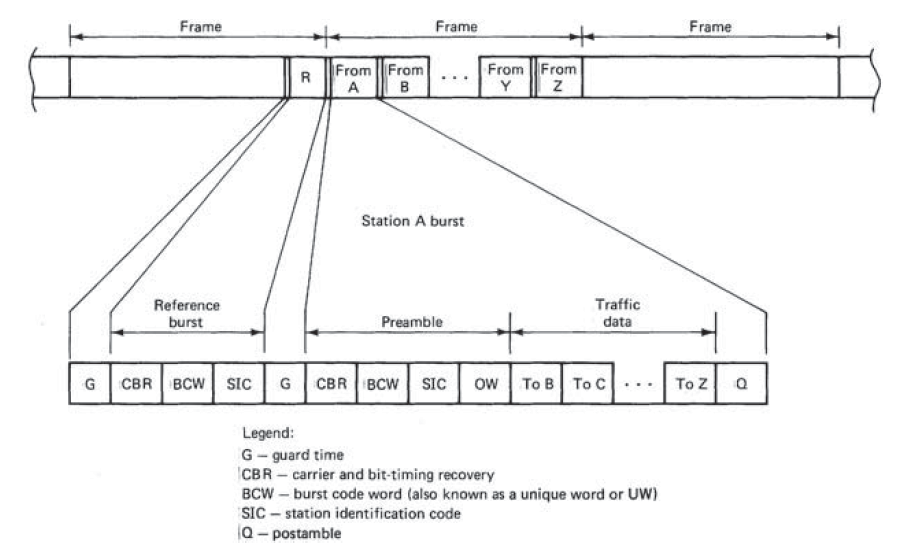
\includegraphics[width=\linewidth]{image6}
  \caption{Frame and burst format in a TDMA system.\cite{Roddy440}}
  \figlabel{Burst_Format}
\end{figure}

\textbf{Traffic Burst: }Traffic bursts are transmitted by different transmitting stations and consist of time slots for the Preamble, actual traffic data, and the Postamble as shown in \figref{Burst_Format}. The \textbf{\textit{preamble}} is the initial segment of a traffic burst, containing information comparable to that found in the reference burst. In certain systems, the channel assignments in both the reference bursts and the preambles are the same. The preamble doesn't transmit any actual traffic.\cite{Roddy440,Roddy451}

In \figref{Burst_Format}, the sole distinction between the preamble and the reference burst is that the preamble includes an \textbf{\textit{orderwire} \textit{(OW) channel}}. The OW channels are used to provide communication such as voice, telegraphy, etc., between earth stations. Like the reference bursts, the preamble serves as a channel for recovering carrier and bit-timing. It also includes a burst-code-word channel for burst-timing purposes. The \textbf{\textit{burst code word}} in the preamble of a traffic burst is distinct from the one in the reference bursts, allowing for the identification of the two types of bursts.

The \textbf{\textit{traffic data}} immediately follows the preamble in a burst. As depicted in \figref{Burst_Format}, the traffic data sub-burst is further divided into time slots designated for individual destination stations. Each destination station selects only the data in the time slots intended for it. The greater the fraction of frame time allocated to traffic, the higher the efficiency. Frame efficiency, a measure of the fraction of frame time used for traffic transmission, can be defined as:
\begin{equation}
Frame\ efficiency({\eta }_F)=\ \frac{traffic\ bits}{total\ bits}
\end{equation}
In certain phase detection systems, there needs to be a pause or recovery time for the phase detector between receiving one burst and the next. This is known as \textbf{\textit{decoder quenching}}, and a designated time slot, referred to as a \textbf{\textit{postamble}}, is allocated for this purpose, labeled as Q in \figref{Burst_Format}.\cite{Roddy440,Roddy451}


\subsection{ Pros and Cons of TDMA systems}
\seclabel{Pros_cons_TDMA}

\noindent One significant benefit of the TDMA mode is that the burst time plan is predominantly controlled by software. This allows for a more flexible adaptation to changes in traffic patterns compared to FDMA, where adjustments often necessitate hardware modifications. Moreover, TDMA offers the following advantages:

\begin{enumerate}

\item  The satellite repeater channel amplifies a single carrier occupying the entire channel bandwidth at any given moment, eliminating intermodulation products. This allows the carrier to maximize the saturation power of the channel.

\item  TDMA maintains high efficiency even with a considerable number of accesses.

\item  Station transmitting power control is unnecessary, streamlining operational requirements.

\item  All stations transmit and receive on the same frequency, irrespective of the burst's origin or destination. This simplifies tuning processes.

\end{enumerate}

\noindent Nevertheless, TDMA comes with certain drawbacks as it is more intricate than FDMA:

\begin{enumerate}
\item  Two reference stations are required, and intricate computer processes are necessary for automated synchronizations.
\item  The peak power and bandwidth requirements for individual earth station terminals need to be larger compared to FDMA due to the high burst bit rate.\cite{Ilcev2013,Roddy445,Maral302}
\end{enumerate}

\section{Code Division Multiple Access (CDMA)}
\seclabel{CDMA}

\noindent The contemporary CDMA approach relies on a modulation method referred to as \textbf{\textit{Spread Spectrum Multiple Access (SSMA)}}. This technique involves distributing the information carried by a specific signal across a significantly broader bandwidth than the original signal. In CDMA, individual carriers can coexist simultaneously within the same RF bandwidth. However, each carrier is distinguished by a unique code waveform, in addition to carrying the information signal.

Regarding the specific encoding procedure, each user is allocated a signature sequence, distinguished by a unique code selected from a set of codes specifically assigned to users in the system. This code is combined, serving as an additional modulation, with the useful information signal. On the receiving end, a particular mobile user can identify and isolate the signal intended for it by using its unique code, thereby extracting the relevant information by performing the correlation technique.\cite{Ilcev2013,Roddy472}


\subsection{ Types of CDMA techniques}
\seclabel{Types_CDMA}

\noindent The Spread Spectrum Multiple Access (SSMA) technique can be categorized into two methods: Direct Sequence (DS) and Frequency Hopping (FH). When both DS and FH are combined in a system, it is referred to as a \textit{hybrid CDMA system}, allowing for an enhancement in processing gain without increasing chip rate.\cite{Ilcev2013}

\textbf{Direct Sequence (DS) CDMA: }The DS-CDMA technique, also known as \textit{Pseudo-Noise (PN) modulation}, involves multiplying the modulated signal by a PN code generator. This generator produces a pseudorandom binary sequence with a length of N at a chip rate (R${}_{c}$), which is considerably higher than the information bit rate (R${}_{b}$). \figref{DS-CDMA} demonstrates the concept for DS-CDMA: the binary message, denoted as m(t), with a bit rate of R${}_{b}$ = 1/T${}_{b}$, is encoded in non-return to zero (NRZ) such that m(t) = $\mathrm{\pm}$1 as shown in figure 4.1. It is then multiplied by a binary sequence, p(t), also coded in NRZ with p(t) = $\mathrm{\pm}$1. The bit rate of the sequence p(t) is R${}_{c}$ = 1/T${}_{c}$, exceeding the bit rate R${}_{b}$ by a factor of 10${}^{2}$--10${}^{6}$. The individual binary elements of the sequence p(t) are referred to as chips, distinguishing them from the message bits. The relation in Equation 6 establishes the chip rate sequence as:
\begin{equation}
{\mathrm{R}}_{\mathrm{c}}\mathrm{=N.}{\mathrm{R}}_{\mathrm{b}}
\end{equation}
\begin{figure}[!h]
\center
  \includegraphics*[width=5.19in, height=4.24in]{image7}
  \caption{Direct Sequence (DS) CDMA.\cite{Maral303}}
  \figlabel{DS-CDMA}
\end{figure}
This sequence is then integrated with the information signal, which is segmented into small chip rates (R${}_{c}$). As a result, this combination accelerates the signal across a much broader bandwidth (W$\mathrm{\sim}$R${}_{c}$). Consequently, the resulting signal possesses a broader RF bandwidth compared to the initial modulated signal as shown in  \figref{Spectrum-CDMA}.\cite{Ilcev2013,Maral303}

\begin{figure}[!h]
\center
  \includegraphics*[width=5.13in, height=1.90in]{image8}
  \caption{Frequency Spectrum of the carrier in DS-CDMA .\cite{Maral303}}
  \figlabel{Spectrum-CDMA}
\end{figure}

The resulting composite signal, m(t)p(t), modulates a carrier using binary phase shift keying (BPSK), with a frequency common to all network stations. The transmitted carrier c(t) can be expressed as:
\begin{equation}
\mathrm{c(t)=m(t)p(t)}{\mathrm{cos} {\omega }_{\mathrm{c}}\mathrm{t}\ }
\end{equation}
At the receiver, coherent demodulation occurs by multiplying the received signal with a replica of the carrier. Neglecting thermal noise, the signal r(t) at the input of the detector low-pass filter (LPF) is given by:
\begin{equation}
\mathrm{r(t)=m(t)p(t)}{\mathrm{cos} {\omega }_{\mathrm{c}}\mathrm{t}\ }\mathrm{\ (2}{\mathrm{cos} {\omega }_{\mathrm{c}}\mathrm{t}\ }\mathrm{)=m(t)p(t)+m(t)p(t)}{\mathrm{cos} {\mathrm{2}\omega }_{\mathrm{c}}\mathrm{t}\ }
\end{equation}
The LPF eliminates high-frequency components at 2${\omega }_{\mathrm{c}}$ and retains only the low-frequency component u(t)=m(t)p(t). This component is then multiplied by the local code p(t) in phase with the received code. In this multiplication, p(t)${}^{2}$=1. At the output of the multiplier, this results in:
\begin{equation}
\mathrm{x(t)=\ m(t)p(t)p(t)=m(t)}{\mathrm{p(t)}}^{\mathrm{2}}\mathrm{=m(t)}
\end{equation}
Subsequently, this signal is integrated over the one-bit period to filter out noise, ultimately recovering the transmitted message m(t) at the integrator output.\cite{Maral303}

\textbf{Frequency Hopping (FH) CDMA: }The FH-CDMA system operates like the DS system, involving a de-hopping correlation process at the receiver. The distinction lies in the utilization of a pseudorandom sequence to manage a frequency synthesizer as shown in  \figref{FH-CDMA}. This leads to the transmission of each information bit rate through multiple pulses at varied frequencies across an expanded bandwidth.\cite{Ilcev2013,Maral303}

\begin{figure}[!h]
\center
  \includegraphics*[scale=0.8]{image9}
  \caption{Frequency Hopping (FH) CDMA. \cite{Maral303}}
  \figlabel{FH-CDMA}
\end{figure}

\subsection{Pros and Cons of CDMA systems}
\seclabel{Pros_cons_CDMA}

\noindent CDMA possesses several advantages:

\begin{enumerate}
\item  \textbf{Simplicity of Operation:} CDMA is straightforward to operate as it doesn't necessitate transmission synchronization among stations. Receiver synchronization is the only requirement, aligning with the received carrier sequence.

\item  \textbf{Interference Resistance:} It provides robust protection against interference from other systems and disturbances caused by multiple paths. This attribute makes it particularly appealing for networks with numerous small stations featuring broad antenna beamwidths and for satellite communication with mobile devices.

\item  \textbf{Frequency Reuse with Multibeam Satellites:} In the context of multibeam satellites, CDMA offers the potential for 100\% frequency reuse between beams.
\end{enumerate}

\noindent However, its primary disadvantage is its relatively low efficiency. The required bandwidth for the space segment of the spread carrier is considerably larger compared to that of a single un-spread carrier, resulting in a somewhat lower throughput compared to other systems. Additionally, CDMA faces limitations related to the finite number of codes, impacting the number of simultaneous users and their inter-correlation properties needed for optimal performance.\cite{Maral314}



\section{ Space Division Multiple Access (SDMA)}
\seclabel{SDMA}
SDMA technology has been effectively utilized in satellite communications for an extended period. SDMA represents a distinctive system access approach, enabling a solitary transmitting site to deliver multiple communication channels. This is achieved by segmenting the radio coverage into focused radio beams that reuse the same frequency. Consequently, it enhances the \textit{signal-to-interference ratio (SIR)}, allowing geographically distant earth stations to access the satellite while utilizing the same frequency.

A solitary satellite has the potential to attain spatial separation through the utilization of beams featuring horizontal and vertical polarization or left-hand and right-hand circular polarization. This enables two beams to encompass the same area on Earth while being differentiated by polarization. Consequently, the satellite could incorporate several beams either through distinct antennas or by employing a single antenna with multiple feeds. In the case of multiple satellites, spatial segregation can be accomplished through differences in orbital longitude or latitude. For inter-satellite connections, separation is achieved by utilizing distinct planes.

In SDMA, two beamforming strategies are employed: \textit{Switched-Beam Antennas}, which individually track subscribers in a cell as they move, and \textit{Adaptive Array Antenna Systems}, which choose a specific beam pattern for each subscriber from a set of preset fixed patterns based on their location.\cite{Ilcev2013,Ilcev2011}

\subsection{Switched Spot Beam Antenna}
\seclabel{Spot}

Switched Multi-Beam Antennas track individual subscribers within a cell using distinct beam patterns. This involves employing array antennas to create overlapping beams for comprehensive coverage. The technique incorporates beam-switching algorithms and RF signal-processing software in smart antenna designs. These algorithms dynamically select beams to maintain optimal signal quality, ensuring customers experience optimal quality throughout their calls. The system periodically scans beam outputs, selecting the one with the highest power. Overlapping beam patterns, as illustrated in \figref{SDMA}(a) with black
cells reuse the frequencies resulting in interference. Therefore, narrow beams are used for reducing it, and as the mobile terminal moves, the smart antenna array monitors the signal strength for selecting the specified beam.\cite{Ilcev2013,Ilcev2011}

\subsection{Adaptive Array Antenna Systems}
\seclabel{Adaptive}

Adaptive array antenna systems continuously analyze their coverage areas, striving to adjust to the dynamic radio environment, including mobile users and potential interferers. In a basic scenario with a single user and no interferers, the system adapts to the user's movement by generating an effective antenna pattern that tracks the user, ensuring maximum gain in their direction. The concept of SDMA with adaptive antenna application differs significantly from the beam-forming methods outlined in \figref{SDMA}(b).\cite{Ilcev2013,Ilcev2011}

\begin{figure}[!h]
\center
  \includegraphics*[scale=0.7]{image10}
  \caption{(a) The beam patterns for the cover of the earth's surface. (b) Adaptive Antenna Applications for SDMA.\cite{Ilcev2011}}
  \figlabel{SDMA}
\end{figure}

\subsection{Advantages of SDMA}
\seclabel{Adv-SDMA}
\begin{enumerate}
\item Significant reduction in the number of cells needed to cover a specific area.

\item Substantial reduction in interference from other systems and users in different cells.

\item Mitigation of the negative effects of multipath signals, often caused by reflections from objects between the signal source and the antenna.

\item Possibility of tighter channel reuse patterns, as average interference from co-channel signals in other cells is markedly decreased.

\item Creation of separate spatial channels within each cell on the same conventional channel, enabling intra-cell reuse of conventional channels.

\item Lower total power radiation from SDMA stations compared to conventional stations, leading to reduced network-wide RF pollution and smaller power amplifier sizes.

\item Knowledge of the direction of each spatial channel, allowing accurate determination of the signal source's position.

\item Compatibility of SDMA with various modulation methods, bandwidths, and frequency bands, including GSM, PHP, DECT, IS-54, IS-95, and other formats. The SDMA solution can be implemented with a wide range of array geometries and antenna types.\cite{Ilcev2013,Ilcev2011}
\end{enumerate}

\section{ Random (Packet) Division Multiple Access (RDMA)}
\seclabel{RDMA}
This access type is ideal for networks with numerous earth stations transmitting short, randomly generated messages with extended silent intervals. It employs random transmission of limited-duration packets without any restrictions, forming bursts occupying all or part of the repeater channel's bandwidth. This method involves time division and random access, allowing message transmission with potential collisions at the satellite. Collisions lead to interference noise, potentially affecting demodulation and message identification, necessitating burst retransmission. Retransmissions may happen multiple times with random delays. This approach involves on-demand competition for satellite resources, assuming no simultaneous access by other transmitters. Random protocols differ in strategies to address this, measured by \textit{throughput} (traffic volume to channel capacity ratio) and \textit{mean transmission delay} (average time from message generation to correct reception).\cite{Ilcev2013,Maral317}

\subsection{ALOHA protocol (Asynchronous protocol)}
\seclabel{ALOHA}
Aloha is a basic mode where multiple users randomly access time-shared a single RF to transmit packets. Upon transmission, a station checks for successful reception through retransmissions from the satellite or acknowledgments from receiving stations. Collisions prompt a random wait before the retransmission of packets. Aloha offers decentralized, cost-effective transmission but has a maximum normalized throughput limit of 18\%, and mean transmission time rises rapidly with increased traffic due to more collisions and packet retransmissions.\cite{Ilcev2013,Maral317}

\subsection{Slotted ALOHA protocol (Synchronous protocol)}
\seclabel{S-ALOHA}

This variant of Aloha, known as S-Aloha or Slotted Aloha, divides time into slots matching a single packet burst. Unlike ordinary Aloha, there is no overlap, and transmissions from various stations are synchronized to specific time slots defined by network clocks, equal to the standard packet duration. This eliminates partial collisions, reducing the timescale of collisions to the duration of a packet, as opposed to Aloha, where it equals the duration of both packets.

This protocol eliminates collisions between new messages and retransmissions, boosting S-Aloha throughput by approximately 50–60\%. It introduces a frame structure with numbered time slots. Each packet includes information indicating the reserved slot number for retransmission in case of collision. Compared to basic Aloha, it improves both time delay and the probability of packet loss for the same utilization value. However, it demands more sophisticated Earth station equipment due to timing requirements, and customers with modest transmission needs may underutilize fixed time slots.\cite{Ilcev2013,Maral317}

\subsection{Slot Reservation Aloha}
\seclabel{Slot-ALOHA}
This extension to the slotted‐Aloha scheme introduces the concept of reserving time slots for Earth station transmission, commonly known as Packed Reserved Multiple Access (PRMA). Slot reservation exists in two forms:
\begin{enumerate}
\item \textbf{Implicit:}Upon successfully transmitting, a station reserves the slot for the duration of its transmission. The network controller then notifies all stations that the slot is open for contention again. However, a station with extensive data to transmit could monopolize the system.
\item \textbf{Explicit:}Each user station can send a reservation request for a time slot before data transmission. A record of slot occupation and reservation requests is maintained, allowing for priority allocation of free time slots. Some form of control, whether by a single or all stations, is essential for managing slot occupancy and reservations.\cite{Ilcev2013,Maral317}
\end{enumerate}

\section{Conclusion}
\seclabel{Con}

In conclusion, the project report explores a spectrum of solutions for addressing the intricate challenge of multiple access to a satellite by a network of stations. The selection of access type is intricately tied to economic considerations, navigating the balance between investment and operational costs against revenue benefits.

For continuous or quasi-continuous carrier transmission, such as in telephone, television, and videoconferencing applications, FDMA, TDMA, and CDMA emerge as suitable choices. The report highlights that in scenarios with significant traffic per carrier and limited accesses (trunking), the simplicity of operation renders FDMA advantageous. Conversely, when dealing with small traffic per carrier and a high number of accesses, the efficiency of TDMA and CDMA outweighs that of FDMA, albeit with higher costs for TDMA earth station equipment. CDMA stands out as a preferred choice for small stations grappling with inter-system interference, despite its lower efficiency. The report also emphasizes the efficiency of SDMA in reusing spectrum across distinct spatial domains, especially critical in bandwidth-limited contexts like cellular networks.

The decision-making process between FDMA and TDMA multiple access also necessitates careful consideration of fixed and on-demand assignment options. Economic factors play a pivotal role, in weighing the revenue gains from increased traffic against the augmented costs associated with on-demand assignment control.

Furthermore, for applications characterized by short messages with random generation and extended silent intervals between messages, the report underscores that random access proves to be the most suitable solution. Overall, the comprehensive insights provided in the report equip stakeholders with valuable perspectives for making informed decisions tailored to specific communication scenarios.

\newpage

\begin{thebibliography}{10}
	\bibitem{Ilcev2013}
	S. D. Ilcev, ``Implementation of Multiple Access Techniques Applicable for Maritime Satellite Communications'', \emph{TransNav, the International Journal on Marine Navigation and Safety of Sea Transportation,} vol. 7, no. 4, pp. 529–540, 2013, doi: 10.12716/1001.07.04.08.
	\bibitem{Ilcev2005}
	S. D. Ilcev,``Global Mobile Satellite Communications for Maritime, Land and Aeronautical Applications,'' Boston: Springer, 2005.
	\bibitem{Roddy423}
	D. Roddy, ``Satellite Communications'', Fourth Edition McGraw-Hill, 2006, pp. 423--424.
	\bibitem{Maral284}
	G. Maral, M. Bousquet, and Z. Sun,``Satellite communications systems: systems, techniques and technology'', Sixth Edition John Wiley \& Sons, 2020, p. 284.
	\bibitem{Maral285}
	G. Maral, M. Bousquet, and Z. Sun,``Satellite communications systems: systems, techniques and technology'', Sixth Edition John Wiley \& Sons, 2020, pp. 285--286.
	\bibitem{Maral286}
	G. Maral, M. Bousquet, and Z. Sun,``Satellite communications systems: systems, techniques and technology'', Sixth Edition John Wiley \& Sons, 2020, pp. 286--288.
	\bibitem{Maral289}
	G. Maral, M. Bousquet, and Z. Sun,``Satellite communications systems: systems, techniques and technology'', Sixth Edition John Wiley \& Sons, 2020, pp. 289--290.
	\bibitem{Roddy436}
	D. Roddy, ``Satellite Communications'', Fourth Edition McGraw-Hill, 2006, pp. 436--439.
	\bibitem{Roddy440}
	D. Roddy, ``Satellite Communications'', Fourth Edition McGraw-Hill, 2006, pp. 440--442.
	\bibitem{Roddy451}
	D. Roddy, ``Satellite Communications'', Fourth Edition McGraw-Hill, 2006, p. 451.
	\bibitem{Roddy445}
	D. Roddy, ``Satellite Communications'', Fourth Edition McGraw-Hill, 2006, pp. 445.
	\bibitem{Maral302}
	G. Maral, M. Bousquet, and Z. Sun,``Satellite communications systems: systems, techniques and technology'', Sixth Edition John Wiley \& Sons, 2020, pp. 302--303.
	\bibitem{Roddy472}
	D. Roddy, ``Satellite Communications'', Fourth Edition McGraw-Hill, 2006, pp. 472.
	\bibitem{Maral303}
	G. Maral, M. Bousquet, and Z. Sun,``Satellite communications systems: systems, techniques and technology'', Sixth Edition John Wiley \& Sons, 2020, pp. 303--306.
	\bibitem{Maral314}
	G. Maral, M. Bousquet, and Z. Sun,``Satellite communications systems: systems, techniques and technology'', Sixth Edition John Wiley \& Sons, 2020, p. 314.
	\bibitem{Ilcev2011}
	S. D. Ilcev, ``Space Division Multiple Access (SDMA) applicable for Mobile Satellite Communications'', \emph{in 2011 10th International Conference on Telecommunication in Modern Satellite Cable and Broadcasting Services (TELSIKS), IEEE}, Oct. 2011, pp. 693–696. doi: 10.1109/TELSKS.2011.6143206.
	\bibitem{Maral317}
	G. Maral, M. Bousquet, and Z. Sun,``Satellite communications systems: systems, techniques and technology'', Sixth Edition John Wiley \& Sons, 2020, pp. 317-322.
	
\end{thebibliography}

\end{lecture}
\theend
